\lfoot{Autor: Raphael Simsek}
\subsection{Schaltvorschlag}
\label{subsec:schaltvorschlag}

\subsubsection{Prototyp}
Für einen Prototyp wurden Schaltkriterien herangezogen.

\begin{itemize}
	\item \glqq 90\% der max. Drehzahl oder Drehmoment erzeugt hochschalten, wegen niedrigem Wirkungsgrad
	\item niedrige Drehzahl und hohe Last erzeugen hinunterschalten, wegen Verschleiß durch Motorschwingungen\grqq
\end{itemize}

Abbildung \ref{fig:imgEngineEfficiencyGraph} zeigt die Umsetzungsüberlegungen am Beginn der Prototypenphase. Dabei ist auf der horizontalen Achse die Drehzahl und auf der vertikalen Achse das Drehmoment abgebildet.
\begin{figure}[!htb]\centering
		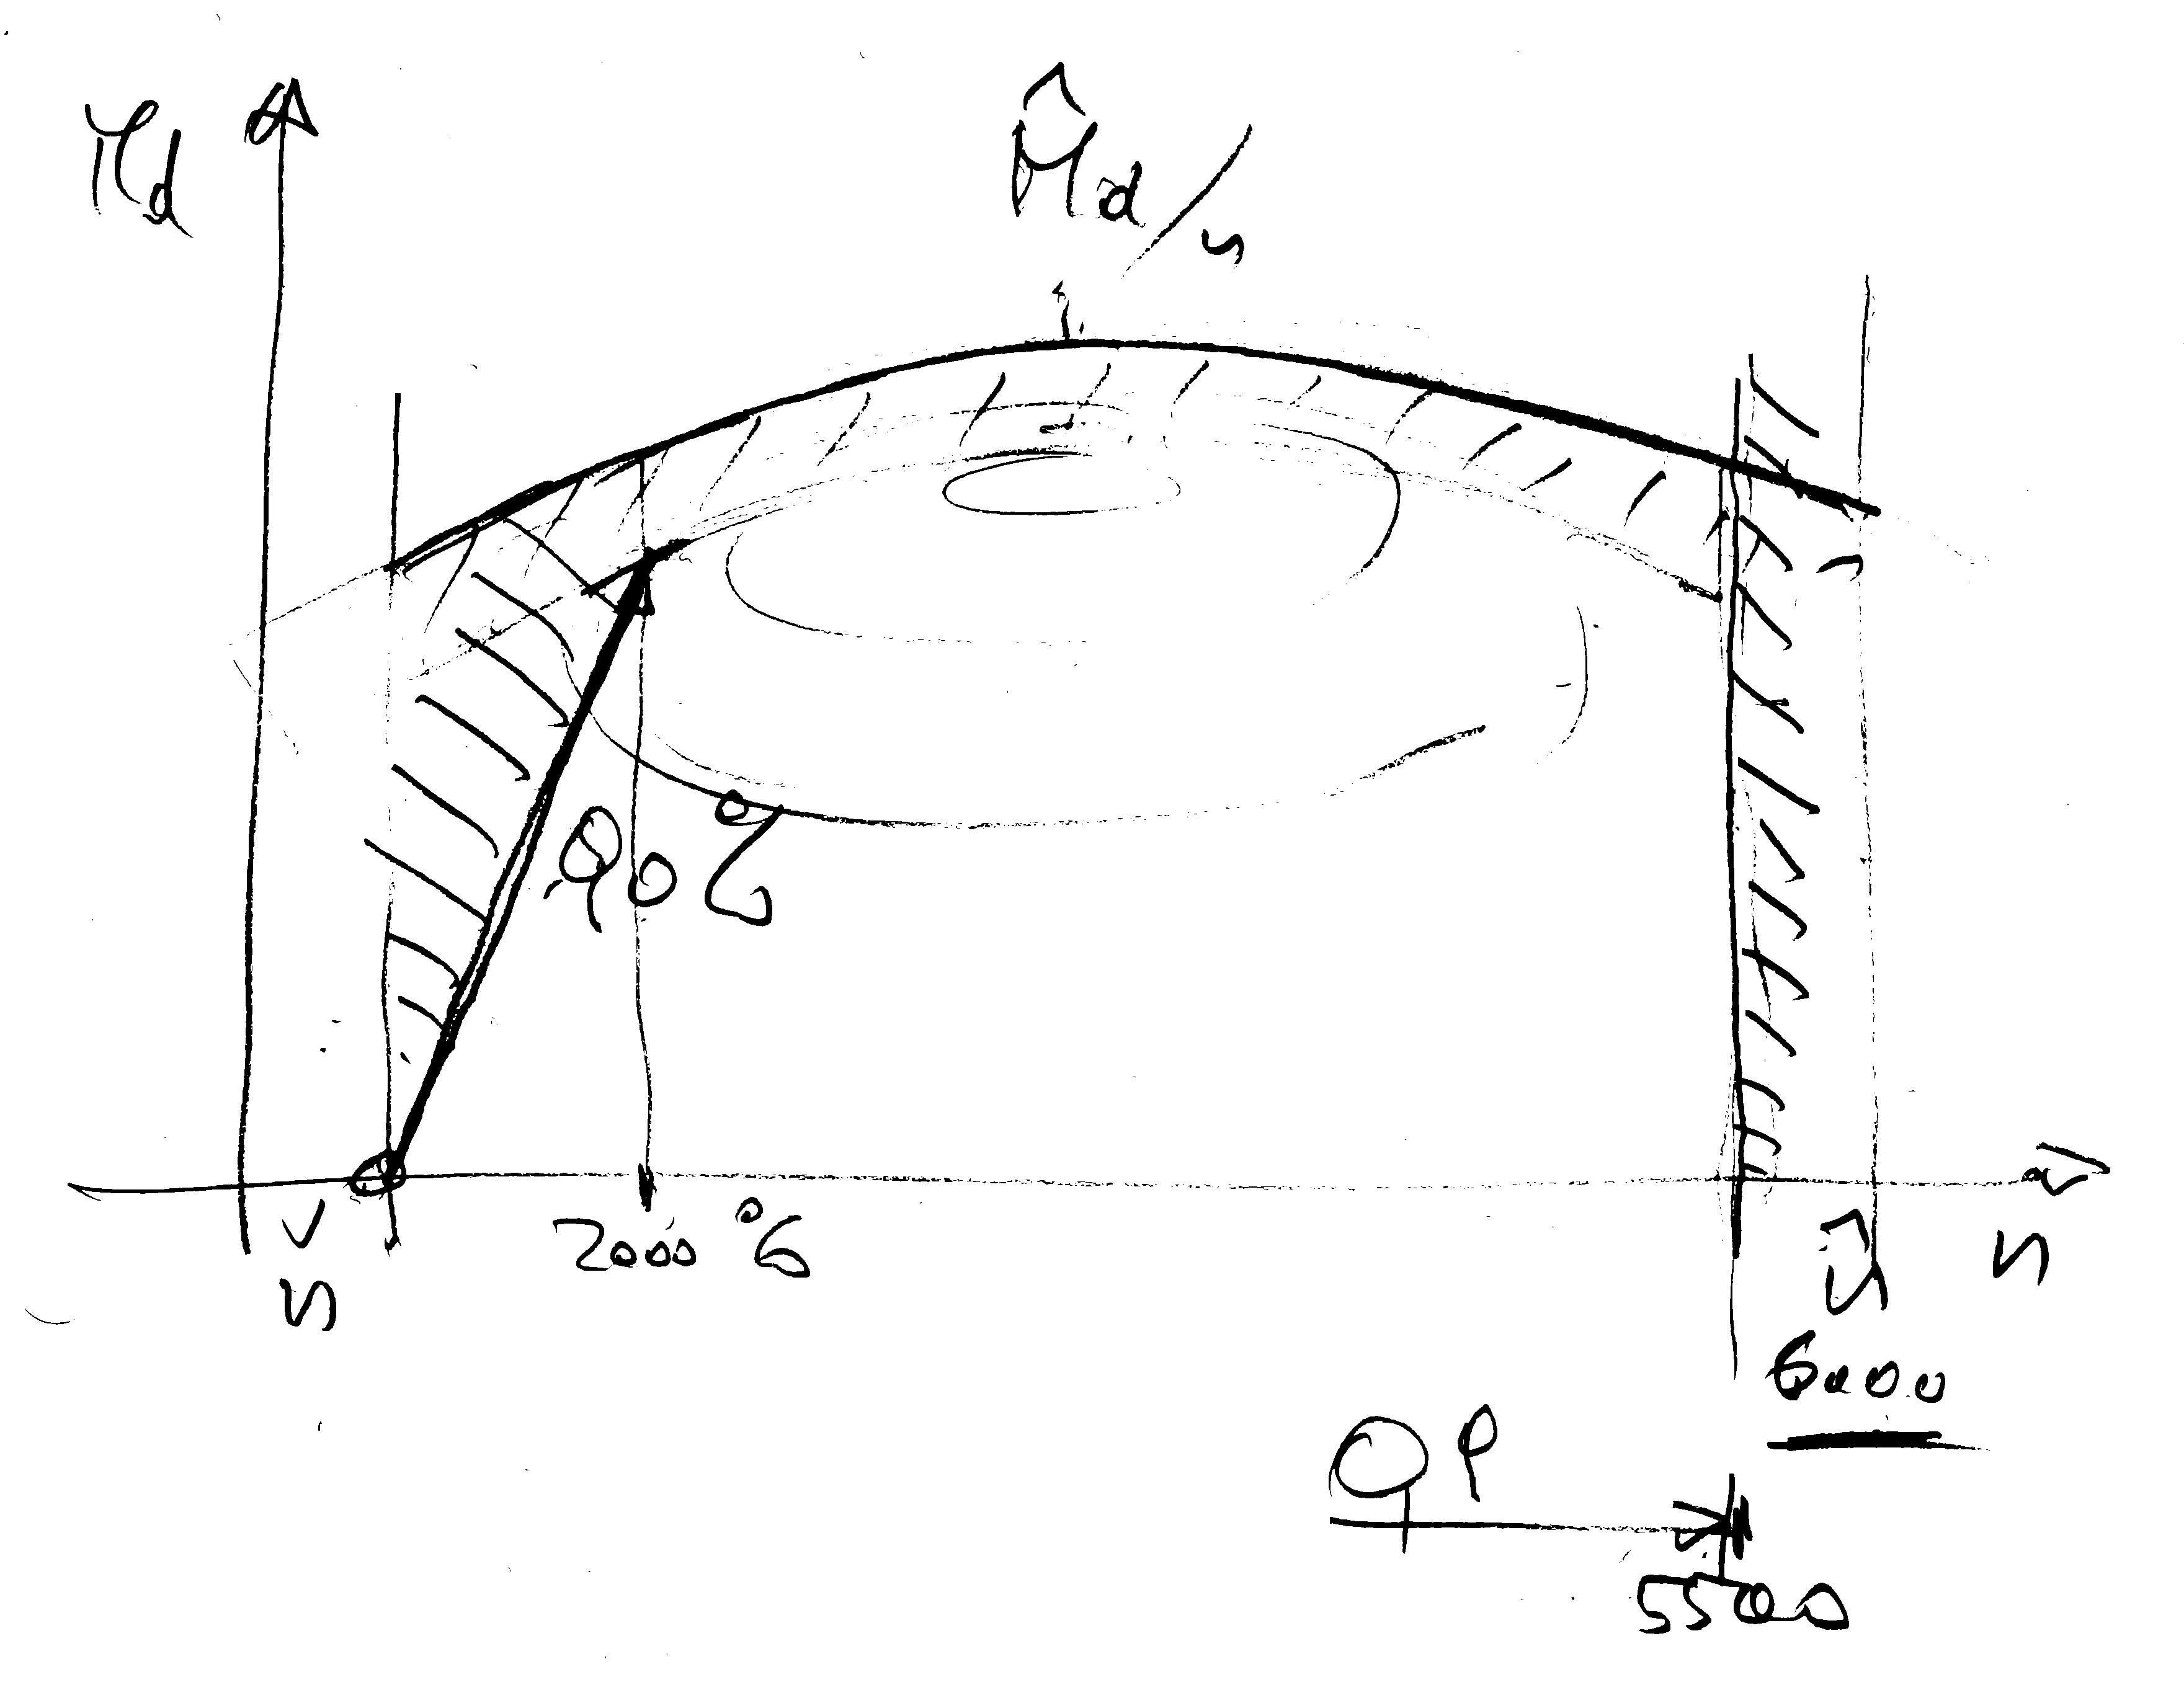
\includegraphics[width=0.75\textwidth]{images/motorkennfeldSkizze}
		\caption{Skizze eines Motorkennfelds} \label{fig:imgEngineEfficiencyGraph}
\end{figure}
Auf Abbildung \ref{fig:imgEngineEfficiencyGraph} ist der Grenzwertbereich für das Hinunterschalten links in Rot, welcher aufgrund des Abriebs des Getriebes ausgelöst wird, erkennbar. Außerdem sind die Grenzwerte für das Hochschalten oben, entlang 90\% des maximalen Drehmoments auf der Drehmomentkurve und rechts entlang 90\% der maximalen Drehzahl in der Farbe Blau, ersichtlich.

Zunächst wurde überprüft, welche PID's Informationen liefern, die für einen Schaltvorschlag notwendig sind. Dazu wird die ODB2-Schnittstelle des KFZ wie in Kapitel \ref{subsec:obd2} beschrieben abgefragt. In Tabelle \ref{tableMazda3} ist das Ergebnis dieser Abfrage für das verwendete Testfahrzeug, ein Mazda 3 BJ 2006, zu sehen. Interessant für einen Schaltvorschlag sind vor allem die PIDs OC - Engine rpm und 04 - calculated engine load, weil diese sich dann auf die Abbildung übertragen lassen und dadurch eine Herleitung zur Implementierung in der Programmierung ermöglichen.

Es wurde festgestellt, dass durch die fehlende Unterstützung für Schaltgetriebe, händisch in einer Settingpane eingegeben werden muss wie hoch die maximale Drehzahl des Motors ist. (Diesel und Benzin stark unterschiedliche maximale Drehzahlen!)

\begin{table}[!htb]
\centering
\resizebox{\columnwidth}{!}{%
\begin{tabular}{lcccccccccccccccccccccccccccccccc}
\cellcolor[HTML]{9B9B9B}Mode 01: 00-20 & \multicolumn{1}{l}{} & \multicolumn{1}{l}{} & \multicolumn{1}{l}{} & \multicolumn{1}{l}{} & \multicolumn{1}{l}{} & \multicolumn{1}{l}{} & \multicolumn{1}{l}{} & \multicolumn{1}{l}{} & \multicolumn{1}{l}{} & \multicolumn{1}{l}{} & \multicolumn{1}{l}{} & \multicolumn{1}{l}{} & \multicolumn{1}{l}{} & \multicolumn{1}{l}{} & \multicolumn{1}{l}{} & \multicolumn{1}{l}{} & \multicolumn{1}{l}{} & \multicolumn{1}{l}{} & \multicolumn{1}{l}{} & \multicolumn{1}{l}{} & \multicolumn{1}{l}{} & \multicolumn{1}{l}{} & \multicolumn{1}{l}{} & \multicolumn{1}{l}{} & \multicolumn{1}{l}{} & \multicolumn{1}{l}{} & \multicolumn{1}{l}{} & \multicolumn{1}{l}{} & \multicolumn{1}{l}{} & \multicolumn{1}{l}{} & \multicolumn{1}{l}{} & \multicolumn{1}{l}{} \\ \hline
\multicolumn{1}{|l|}{Hexadecimal} & \multicolumn{4}{c|}{B} & \multicolumn{4}{c|}{E} & \multicolumn{4}{c|}{3} & \multicolumn{4}{c|}{F} & \multicolumn{4}{c|}{A} & \multicolumn{4}{c|}{8} & \multicolumn{4}{c|}{1} & \multicolumn{4}{c|}{3} \\ \hline
\multicolumn{1}{|l|}{Binary} & \multicolumn{1}{c|}{1} & \multicolumn{1}{c|}{0} & \multicolumn{1}{c|}{1} & \multicolumn{1}{c|}{1} & \multicolumn{1}{c|}{1} & \multicolumn{1}{c|}{1} & \multicolumn{1}{c|}{1} & \multicolumn{1}{c|}{0} & \multicolumn{1}{c|}{\cellcolor[HTML]{FFFFFF}0} & \multicolumn{1}{c|}{0} & \multicolumn{1}{c|}{1} & \multicolumn{1}{c|}{1} & \multicolumn{1}{c|}{1} & \multicolumn{1}{c|}{\cellcolor[HTML]{FFFFFF}1} & \multicolumn{1}{c|}{1} & \multicolumn{1}{c|}{1} & \multicolumn{1}{c|}{\cellcolor[HTML]{9AFF99}1} & \multicolumn{1}{c|}{0} & \multicolumn{1}{c|}{1} & \multicolumn{1}{c|}{0} & \multicolumn{1}{c|}{1} & \multicolumn{1}{c|}{0} & \multicolumn{1}{c|}{0} & \multicolumn{1}{c|}{0} & \multicolumn{1}{c|}{0} & \multicolumn{1}{c|}{0} & \multicolumn{1}{c|}{0} & \multicolumn{1}{c|}{1} & \multicolumn{1}{c|}{0} & \multicolumn{1}{c|}{0} & \multicolumn{1}{c|}{1} & \multicolumn{1}{c|}{1} \\ \hline
\multicolumn{1}{|l|}{Supported?} & \multicolumn{1}{c|}{\cellcolor[HTML]{9AFF99}Yes} & \multicolumn{1}{c|}{\cellcolor[HTML]{FD6864}No} & \multicolumn{1}{c|}{\cellcolor[HTML]{9AFF99}Yes} & \multicolumn{1}{c|}{\cellcolor[HTML]{9AFF99}Yes} & \multicolumn{1}{c|}{\cellcolor[HTML]{9AFF99}Yes} & \multicolumn{1}{c|}{\cellcolor[HTML]{9AFF99}Yes} & \multicolumn{1}{c|}{\cellcolor[HTML]{9AFF99}Yes} & \multicolumn{1}{c|}{\cellcolor[HTML]{FD6864}No} & \multicolumn{1}{c|}{\cellcolor[HTML]{FD6864}No} & \multicolumn{1}{c|}{\cellcolor[HTML]{FD6864}No} & \multicolumn{1}{c|}{\cellcolor[HTML]{9AFF99}Yes} & \multicolumn{1}{c|}{\cellcolor[HTML]{9AFF99}Yes} & \multicolumn{1}{c|}{\cellcolor[HTML]{9AFF99}Yes} & \multicolumn{1}{c|}{\cellcolor[HTML]{9AFF99}Yes} & \multicolumn{1}{c|}{\cellcolor[HTML]{9AFF99}Yes} & \multicolumn{1}{c|}{\cellcolor[HTML]{9AFF99}Yes} & \multicolumn{1}{c|}{\cellcolor[HTML]{9AFF99}Yes} & \multicolumn{1}{c|}{\cellcolor[HTML]{FD6864}No} & \multicolumn{1}{c|}{\cellcolor[HTML]{9AFF99}Yes} & \multicolumn{1}{c|}{\cellcolor[HTML]{FD6864}No} & \multicolumn{1}{c|}{\cellcolor[HTML]{9AFF99}Yes} & \multicolumn{1}{c|}{\cellcolor[HTML]{FD6864}No} & \multicolumn{1}{c|}{\cellcolor[HTML]{FD6864}No} & \multicolumn{1}{c|}{\cellcolor[HTML]{FD6864}No} & \multicolumn{1}{c|}{\cellcolor[HTML]{FD6864}No} & \multicolumn{1}{c|}{\cellcolor[HTML]{FD6864}No} & \multicolumn{1}{c|}{\cellcolor[HTML]{FD6864}No} & \multicolumn{1}{c|}{\cellcolor[HTML]{9AFF99}Yes} & \multicolumn{1}{c|}{\cellcolor[HTML]{FD6864}No} & \multicolumn{1}{c|}{\cellcolor[HTML]{FD6864}No} & \multicolumn{1}{c|}{\cellcolor[HTML]{9AFF99}Yes} & \multicolumn{1}{c|}{\cellcolor[HTML]{9AFF99}Yes} \\ \hline
\multicolumn{1}{|l|}{PID number} & \multicolumn{1}{c|}{1} & \multicolumn{1}{c|}{2} & \multicolumn{1}{c|}{3} & \multicolumn{1}{c|}{4} & \multicolumn{1}{c|}{5} & \multicolumn{1}{c|}{6} & \multicolumn{1}{c|}{7} & \multicolumn{1}{c|}{8} & \multicolumn{1}{c|}{9} & \multicolumn{1}{c|}{0A} & \multicolumn{1}{c|}{0B} & \multicolumn{1}{c|}{0C} & \multicolumn{1}{c|}{0D} & \multicolumn{1}{c|}{0E} & \multicolumn{1}{c|}{0F} & \multicolumn{1}{c|}{10} & \multicolumn{1}{c|}{11} & \multicolumn{1}{c|}{12} & \multicolumn{1}{c|}{13} & \multicolumn{1}{c|}{14} & \multicolumn{1}{c|}{15} & \multicolumn{1}{c|}{16} & \multicolumn{1}{c|}{17} & \multicolumn{1}{c|}{18} & \multicolumn{1}{c|}{19} & \multicolumn{1}{c|}{1A} & \multicolumn{1}{c|}{1B} & \multicolumn{1}{c|}{1C} & \multicolumn{1}{c|}{1D} & \multicolumn{1}{c|}{1E} & \multicolumn{1}{c|}{1F} & \multicolumn{1}{c|}{20} \\ \hline
\cellcolor[HTML]{9B9B9B}Mode 01: 20-40 & \multicolumn{1}{l}{} & \multicolumn{1}{l}{} & \multicolumn{1}{l}{} & \multicolumn{1}{l}{} & \multicolumn{1}{l}{} & \multicolumn{1}{l}{} & \multicolumn{1}{l}{} & \multicolumn{1}{l}{} & \multicolumn{1}{l}{} & \multicolumn{1}{l}{} & \multicolumn{1}{l}{} & \multicolumn{1}{l}{} & \multicolumn{1}{l}{} & \multicolumn{1}{l}{\cellcolor[HTML]{FFFFFF}} & \multicolumn{1}{l}{} & \multicolumn{1}{l}{} & \multicolumn{1}{l}{} & \multicolumn{1}{l}{} & \multicolumn{1}{l}{} & \multicolumn{1}{l}{} & \multicolumn{1}{l}{} & \multicolumn{1}{l}{} & \multicolumn{1}{l}{} & \multicolumn{1}{l}{} & \multicolumn{1}{l}{} & \multicolumn{1}{l}{} & \multicolumn{1}{l}{} & \multicolumn{1}{l}{} & \multicolumn{1}{l}{} & \multicolumn{1}{l}{} & \multicolumn{1}{l}{} & \multicolumn{1}{l}{} \\ \hline
\multicolumn{1}{|l|}{Hexadecimal} & \multicolumn{4}{c|}{8} & \multicolumn{4}{c|}{0} & \multicolumn{4}{c|}{1} & \multicolumn{4}{c|}{5} & \multicolumn{4}{c|}{B} & \multicolumn{4}{c|}{0} & \multicolumn{4}{c|}{1} & \multicolumn{4}{c|}{1} \\ \hline
\multicolumn{1}{|l|}{Binary} & \multicolumn{1}{c|}{1} & \multicolumn{1}{c|}{0} & \multicolumn{1}{c|}{0} & \multicolumn{1}{c|}{0} & \multicolumn{1}{c|}{0} & \multicolumn{1}{c|}{0} & \multicolumn{1}{c|}{0} & \multicolumn{1}{c|}{0} & \multicolumn{1}{c|}{0} & \multicolumn{1}{c|}{0} & \multicolumn{1}{c|}{0} & \multicolumn{1}{c|}{1} & \multicolumn{1}{c|}{0} & \multicolumn{1}{c|}{1} & \multicolumn{1}{c|}{0} & \multicolumn{1}{c|}{1} & \multicolumn{1}{c|}{1} & \multicolumn{1}{c|}{0} & \multicolumn{1}{c|}{1} & \multicolumn{1}{c|}{1} & \multicolumn{1}{c|}{0} & \multicolumn{1}{c|}{0} & \multicolumn{1}{c|}{0} & \multicolumn{1}{c|}{0} & \multicolumn{1}{c|}{0} & \multicolumn{1}{c|}{0} & \multicolumn{1}{c|}{0} & \multicolumn{1}{c|}{1} & \multicolumn{1}{c|}{0} & \multicolumn{1}{c|}{0} & \multicolumn{1}{c|}{0} & \multicolumn{1}{c|}{1} \\ \hline
\multicolumn{1}{|l|}{Supported?} & \multicolumn{1}{c|}{\cellcolor[HTML]{9AFF99}Yes} & \multicolumn{1}{c|}{\cellcolor[HTML]{FD6864}No} & \multicolumn{1}{c|}{\cellcolor[HTML]{FD6864}No} & \multicolumn{1}{c|}{\cellcolor[HTML]{FD6864}No} & \multicolumn{1}{c|}{\cellcolor[HTML]{FD6864}No} & \multicolumn{1}{c|}{\cellcolor[HTML]{FD6864}No} & \multicolumn{1}{c|}{\cellcolor[HTML]{FD6864}No} & \multicolumn{1}{c|}{\cellcolor[HTML]{FD6864}No} & \multicolumn{1}{c|}{\cellcolor[HTML]{FD6864}No} & \multicolumn{1}{c|}{\cellcolor[HTML]{FD6864}No} & \multicolumn{1}{c|}{\cellcolor[HTML]{FD6864}No} & \multicolumn{1}{c|}{\cellcolor[HTML]{9AFF99}Yes} & \multicolumn{1}{c|}{\cellcolor[HTML]{FD6864}No} & \multicolumn{1}{c|}{\cellcolor[HTML]{9AFF99}Yes} & \multicolumn{1}{c|}{\cellcolor[HTML]{FD6864}No} & \multicolumn{1}{c|}{\cellcolor[HTML]{9AFF99}Yes} & \multicolumn{1}{c|}{\cellcolor[HTML]{9AFF99}Yes} & \multicolumn{1}{c|}{\cellcolor[HTML]{FD6864}No} & \multicolumn{1}{c|}{\cellcolor[HTML]{9AFF99}Yes} & \multicolumn{1}{c|}{\cellcolor[HTML]{9AFF99}Yes} & \multicolumn{1}{c|}{\cellcolor[HTML]{FD6864}No} & \multicolumn{1}{c|}{\cellcolor[HTML]{FD6864}No} & \multicolumn{1}{c|}{\cellcolor[HTML]{FD6864}No} & \multicolumn{1}{c|}{\cellcolor[HTML]{FD6864}No} & \multicolumn{1}{c|}{\cellcolor[HTML]{FD6864}No} & \multicolumn{1}{c|}{\cellcolor[HTML]{FD6864}No} & \multicolumn{1}{c|}{\cellcolor[HTML]{FD6864}No} & \multicolumn{1}{c|}{\cellcolor[HTML]{9AFF99}Yes} & \multicolumn{1}{c|}{\cellcolor[HTML]{FD6864}No} & \multicolumn{1}{c|}{\cellcolor[HTML]{FD6864}No} & \multicolumn{1}{c|}{\cellcolor[HTML]{FD6864}No} & \multicolumn{1}{c|}{\cellcolor[HTML]{9AFF99}Yes} \\ \hline
\multicolumn{1}{|l|}{PID number} & \multicolumn{1}{c|}{21} & \multicolumn{1}{c|}{22} & \multicolumn{1}{c|}{23} & \multicolumn{1}{c|}{24} & \multicolumn{1}{c|}{25} & \multicolumn{1}{c|}{26} & \multicolumn{1}{c|}{27} & \multicolumn{1}{c|}{28} & \multicolumn{1}{c|}{29} & \multicolumn{1}{c|}{2a} & \multicolumn{1}{c|}{2b} & \multicolumn{1}{c|}{2c} & \multicolumn{1}{c|}{2d} & \multicolumn{1}{c|}{2e} & \multicolumn{1}{c|}{2f} & \multicolumn{1}{c|}{30} & \multicolumn{1}{c|}{31} & \multicolumn{1}{c|}{32} & \multicolumn{1}{c|}{33} & \multicolumn{1}{c|}{34} & \multicolumn{1}{c|}{35} & \multicolumn{1}{c|}{36} & \multicolumn{1}{c|}{37} & \multicolumn{1}{c|}{38} & \multicolumn{1}{c|}{39} & \multicolumn{1}{c|}{3a} & \multicolumn{1}{c|}{3b} & \multicolumn{1}{c|}{3c} & \multicolumn{1}{c|}{3d} & \multicolumn{1}{c|}{3e} & \multicolumn{1}{c|}{3f} & \multicolumn{1}{c|}{40} \\ \hline
\cellcolor[HTML]{9B9B9B}Mode 01: 40-60 & \multicolumn{1}{l}{} & \multicolumn{1}{l}{} & \multicolumn{1}{l}{} & \multicolumn{1}{l}{} & \multicolumn{1}{l}{} & \multicolumn{1}{l}{} & \multicolumn{1}{l}{} & \multicolumn{1}{l}{} & \multicolumn{1}{l}{} & \multicolumn{1}{l}{} & \multicolumn{1}{l}{} & \multicolumn{1}{l}{} & \multicolumn{1}{l}{} & \multicolumn{1}{l}{} & \multicolumn{1}{l}{} & \multicolumn{1}{l}{} & \multicolumn{1}{l}{} & \multicolumn{1}{l}{} & \multicolumn{1}{l}{} & \multicolumn{1}{l}{} & \multicolumn{1}{l}{} & \multicolumn{1}{l}{} & \multicolumn{1}{l}{} & \multicolumn{1}{l}{} & \multicolumn{1}{l}{} & \multicolumn{1}{l}{} & \multicolumn{1}{l}{} & \multicolumn{1}{l}{} & \multicolumn{1}{l}{} & \multicolumn{1}{l}{} & \multicolumn{1}{l}{} & \multicolumn{1}{l}{} \\ \hline
\multicolumn{1}{|l|}{Hexadecimal} & \multicolumn{4}{c|}{F} & \multicolumn{4}{c|}{A} & \multicolumn{4}{c|}{D} & \multicolumn{4}{c|}{0} & \multicolumn{4}{c|}{0} & \multicolumn{4}{c|}{0} & \multicolumn{4}{c|}{0} & \multicolumn{4}{c|}{0} \\ \hline
\multicolumn{1}{|l|}{Binary} & \multicolumn{1}{c|}{1} & \multicolumn{1}{c|}{1} & \multicolumn{1}{c|}{1} & \multicolumn{1}{c|}{1} & \multicolumn{1}{c|}{1} & \multicolumn{1}{c|}{0} & \multicolumn{1}{c|}{1} & \multicolumn{1}{c|}{0} & \multicolumn{1}{c|}{1} & \multicolumn{1}{c|}{1} & \multicolumn{1}{c|}{0} & \multicolumn{1}{c|}{1} & \multicolumn{1}{c|}{0} & \multicolumn{1}{c|}{0} & \multicolumn{1}{c|}{0} & \multicolumn{1}{c|}{0} & \multicolumn{1}{c|}{0} & \multicolumn{1}{c|}{0} & \multicolumn{1}{c|}{0} & \multicolumn{1}{c|}{0} & \multicolumn{1}{c|}{0} & \multicolumn{1}{c|}{0} & \multicolumn{1}{c|}{0} & \multicolumn{1}{c|}{0} & \multicolumn{1}{c|}{0} & \multicolumn{1}{c|}{0} & \multicolumn{1}{c|}{0} & \multicolumn{1}{c|}{0} & \multicolumn{1}{c|}{0} & \multicolumn{1}{c|}{0} & \multicolumn{1}{c|}{0} & \multicolumn{1}{c|}{0} \\ \hline
\multicolumn{1}{|l|}{Supported?} & \multicolumn{1}{c|}{\cellcolor[HTML]{9AFF99}Yes} & \multicolumn{1}{c|}{\cellcolor[HTML]{9AFF99}Yes} & \multicolumn{1}{c|}{\cellcolor[HTML]{9AFF99}Yes} & \multicolumn{1}{c|}{\cellcolor[HTML]{9AFF99}Yes} & \multicolumn{1}{c|}{\cellcolor[HTML]{9AFF99}Yes} & \multicolumn{1}{c|}{\cellcolor[HTML]{FD6864}No} & \multicolumn{1}{c|}{\cellcolor[HTML]{9AFF99}Yes} & \multicolumn{1}{c|}{\cellcolor[HTML]{FD6864}No} & \multicolumn{1}{c|}{\cellcolor[HTML]{9AFF99}Yes} & \multicolumn{1}{c|}{\cellcolor[HTML]{9AFF99}Yes} & \multicolumn{1}{c|}{\cellcolor[HTML]{FD6864}No} & \multicolumn{1}{c|}{\cellcolor[HTML]{9AFF99}Yes} & \multicolumn{1}{c|}{\cellcolor[HTML]{FD6864}No} & \multicolumn{1}{c|}{\cellcolor[HTML]{FD6864}No} & \multicolumn{1}{c|}{\cellcolor[HTML]{FD6864}No} & \multicolumn{1}{c|}{\cellcolor[HTML]{FD6864}No} & \multicolumn{1}{c|}{\cellcolor[HTML]{FD6864}No} & \multicolumn{1}{c|}{\cellcolor[HTML]{FD6864}No} & \multicolumn{1}{c|}{\cellcolor[HTML]{FD6864}No} & \multicolumn{1}{c|}{\cellcolor[HTML]{FD6864}No} & \multicolumn{1}{c|}{\cellcolor[HTML]{FD6864}No} & \multicolumn{1}{c|}{\cellcolor[HTML]{FD6864}No} & \multicolumn{1}{c|}{\cellcolor[HTML]{FD6864}No} & \multicolumn{1}{c|}{\cellcolor[HTML]{FD6864}No} & \multicolumn{1}{c|}{\cellcolor[HTML]{FD6864}No} & \multicolumn{1}{c|}{\cellcolor[HTML]{FD6864}No} & \multicolumn{1}{c|}{\cellcolor[HTML]{FD6864}No} & \multicolumn{1}{c|}{\cellcolor[HTML]{FD6864}No} & \multicolumn{1}{c|}{\cellcolor[HTML]{FD6864}No} & \multicolumn{1}{c|}{\cellcolor[HTML]{FD6864}No} & \multicolumn{1}{c|}{\cellcolor[HTML]{FD6864}No} & \multicolumn{1}{c|}{\cellcolor[HTML]{FD6864}No} \\ \hline
\multicolumn{1}{|l|}{PID number} & \multicolumn{1}{c|}{41} & \multicolumn{1}{c|}{42} & \multicolumn{1}{c|}{43} & \multicolumn{1}{c|}{44} & \multicolumn{1}{c|}{45} & \multicolumn{1}{c|}{46} & \multicolumn{1}{c|}{47} & \multicolumn{1}{c|}{48} & \multicolumn{1}{c|}{49} & \multicolumn{1}{c|}{4a} & \multicolumn{1}{c|}{4b} & \multicolumn{1}{c|}{4c} & \multicolumn{1}{c|}{4d} & \multicolumn{1}{c|}{4e} & \multicolumn{1}{c|}{4f} & \multicolumn{1}{c|}{50} & \multicolumn{1}{c|}{51} & \multicolumn{1}{c|}{52} & \multicolumn{1}{c|}{53} & \multicolumn{1}{c|}{54} & \multicolumn{1}{c|}{55} & \multicolumn{1}{c|}{56} & \multicolumn{1}{c|}{57} & \multicolumn{1}{c|}{58} & \multicolumn{1}{c|}{59} & \multicolumn{1}{c|}{5a} & \multicolumn{1}{c|}{5b} & \multicolumn{1}{c|}{5c} & \multicolumn{1}{c|}{5d} & \multicolumn{1}{c|}{5e} & \multicolumn{1}{c|}{5f} & \multicolumn{1}{c|}{60} \\ \hline
\cellcolor[HTML]{9B9B9B}Mode 01: 60-100 & \multicolumn{1}{l}{} & \multicolumn{1}{l}{} & \multicolumn{1}{l}{} & \multicolumn{1}{l}{} & \multicolumn{1}{l}{} & \multicolumn{1}{l}{} & \multicolumn{1}{l}{} & \multicolumn{1}{l}{} & \multicolumn{1}{l}{} & \multicolumn{1}{l}{} & \multicolumn{1}{l}{} & \multicolumn{1}{l}{} & \multicolumn{1}{l}{} & \multicolumn{1}{l}{} & \multicolumn{1}{l}{} & \multicolumn{1}{l}{} & \multicolumn{1}{l}{} & \multicolumn{1}{l}{} & \multicolumn{1}{l}{} & \multicolumn{1}{l}{} & \multicolumn{1}{l}{} & \multicolumn{1}{l}{} & \multicolumn{1}{l}{} & \multicolumn{1}{l}{} & \multicolumn{1}{l}{} & \multicolumn{1}{l}{} & \multicolumn{1}{l}{} & \multicolumn{1}{l}{} & \multicolumn{1}{l}{} & \multicolumn{1}{l}{} & \multicolumn{1}{l}{} & \multicolumn{1}{l}{} \\ \cline{1-1}
\multicolumn{1}{|l|}{NO DATA} & \multicolumn{1}{l}{} & \multicolumn{1}{l}{} & \multicolumn{1}{l}{} & \multicolumn{1}{l}{} & \multicolumn{1}{l}{} & \multicolumn{1}{l}{} & \multicolumn{1}{l}{} & \multicolumn{1}{l}{} & \multicolumn{1}{l}{} & \multicolumn{1}{l}{} & \multicolumn{1}{l}{} & \multicolumn{1}{l}{} & \multicolumn{1}{l}{} & \multicolumn{1}{l}{} & \multicolumn{1}{l}{} & \multicolumn{1}{l}{} & \multicolumn{1}{l}{} & \multicolumn{1}{l}{} & \multicolumn{1}{l}{} & \multicolumn{1}{l}{} & \multicolumn{1}{l}{} & \multicolumn{1}{l}{} & \multicolumn{1}{l}{} & \multicolumn{1}{l}{} & \multicolumn{1}{l}{} & \multicolumn{1}{l}{} & \multicolumn{1}{l}{} & \multicolumn{1}{l}{} & \multicolumn{1}{l}{} & \multicolumn{1}{l}{} & \multicolumn{1}{l}{} & \multicolumn{1}{l}{} \\ \cline{1-1}
\end{tabular}}
\caption{Tabelle der verfügbaren PIDs eines Mazda3}
\label{tableMazda3}
\end{table}
Bei genauerer Betrachtung der PIDs wurde der ursprüngliche Plan, den aktuell eingelegten und den zu wählenden Gang anzuzeigen verworfen, da sich diese Informationen nur mit sehr hohem Aufwand, wenn überhaupt aus den vorhanden Daten ableiten lässt. Eine zusätzliche Sensorik am Getriebe wäre eine mögliche Option gewesen, widerspricht aber - neben rechtlichen Bedenken - dem Ziel des Projektes, die Integration des Car-PCs so einfach wie möglich zu gestalten. Stattdessen einigte sich das Team darauf, sich nur mit einem Vorschlag nach oben oder unten zufrieden zu geben. 

Zum Zweck des Gangvorschlags werden 2 PID's benötigt.
\begin{itemize}
	\item Mode 01 PID 04: calculated engine load [\%]
	\item Mode 01 PID 0C: engine rpm [0-16.383,75]
\end{itemize} 

Durch diese Variablen muss eine Klassenbildung für das herunterschalten umgesetzt werden, da es hier kein einzelnes Maß gibt auf welches man ein überschreiten des Maximums schließen könnte. Beim Heraufschalten, wird keine Klassenbildung benötigt da hier immer entweder zuerst 90\% des möglichen Drehmoments oder der nötigen Drehzahl eintreffen. Der vom Fahrzeug gesammelte Wert der calculated engine load (PID 04) wird bereits als Prozentsatz geliefert.
\subsubsection{Optisches Design der App} 
Bei der Designüberlegung wurde vor allem beachtet, dass das Design so einfach zu bedienen sein sollte. Dies hatte den Zweck möglichst wenig des Fahrers Aufmerksamkeit zu benötigen. Weiters müssen durch die fehlende Unterstützung für Schaltgetriebe der OBD-II Schnittstelle, händisch manche Konstanten in einer Settingpane eingegeben werden. Zusätzlich dazu wurde überlegt, wie man am intuitivsten hinauf oder hinunterschalten anzeigt.


Trotzem viele Fahrzeuge einen Drehzahlmesser im Armaturenbrett integriert haben, wurde eine Drehzahlanzeige neben dem Schaltsymbol platziert. Dadurch bekommt ein Fahranfänger selbst ein Gefühl für das Schalten und sich auf Dauer merken wird in welchen Gang er wann schalten sollte. Ein Aufwärtspfeil symbolisiert einen Schaltvorschlag für einen höheren Gang, ein Abwärtspfeil rät zum Hinunterschalten. Ist keine Aktion gefordert wird eine X angezeigt.

\subsubsection{Umsetzung}
Unsere verbaute Technik ist weitaus moderner als gängige ECUs, welche 10 Jahre oder älter sind. Daher ist auch das Auslesen der Schnittstelle sehr einfach zu handhaben. Als direkte Konkurrenz innerhalb dieser Produktkategorie war kein Produkt auffindbar.
Im Bezug auf meinen Lösungsweg des Schaltvorschlags war ich sehr eingeschränkt, da ich nur den Lösungsweg, welchen mir Prof. Neuburger näher gebracht hat, einsetzen konnte. Dies ist vor allem meinen kaum vorhandenen Fahrzeugtechnik Kenntnissen zu verdanken. Daher habe ich mich dafür entschieden bei dem Ansatz, welchen mir Herr Prof. Neuburger mehr als nur einmal half zu verstehen, zu bleiben. Bezüglich der Android App hatte ich andererseits vollkommene gestalterische Freiheit, hier wurden die Ansätze gewählt, welche am besten dokumentiert sind.
Um diese beiden Teile zu realisieren, wurden mehrere Libraries verwendet, die alle ausschließlich Android Studio verwenden.
Einerseits wurde GaugeView for Lollipop \cite{SIMR.CH3-schaltvorschlag.GaugeView} verwendet, andererseits wurde mittels ImageCircleView \cite{SIMR.CH3-schaltvorschlag.CircleImageView} das Bild des Pfeils und des Kreuzes dargestellt.
Ausserdem musste eine SettingsPane umgesetzt werden, in welcher man die maximale Drehzahl verstellen kann, implementiert werden.
Es wurde die App mittels Gradle und der Android SDK 23 umgesetzt.

Probleme kamen vor allem beim Aufbau der GaugeView Library auf, welche aufgrund eines doppelten XML attributes (showText) händisch zu einem Android Library Package (.aar) kompiliert werden musste, damit dieser Fehler umgangen werden konnte. Ein Patch für die Library wurde bisweilen noch nicht vom Library-Ersteller bereitet (siehe Code Snippet \ref{codeShiftFile}).

\lstinputlisting[caption={Implementierung der GaugeView Library im design.xml},label={codeShiftFile},firstline=11,lastline=26,style=xmlstyle]{code/CH3/schalt.xml}

\lstinputlisting[caption={Implementierung der GaugeView Library im build.gradle},label={codeGradleFile},firstline=42,lastline=46,style=javastyle]{code/CH3/schalt.xml}

\begin{figure}[!htb]\centering
		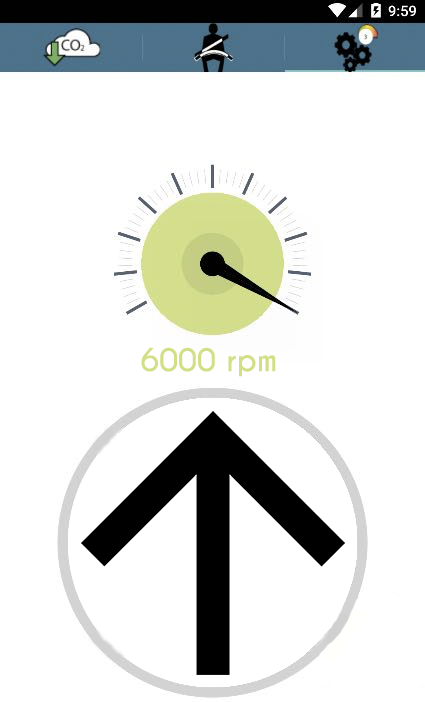
\includegraphics[width=0.3\textwidth]{images/schalt}
		\caption{finale Optik der Android App beim Schaltvorschlag} \label{fig:imgShiftAndroidFinished}
\end{figure}


\clearpage % DO NOT REMOVE